\documentclass[10pt, aspectratio=169, compress]{beamer}
\usetheme[progressbar=frame title, numbering=fraction]{metropolis}      % Use metropolis theme 
\setbeamertemplate{section in toc}[sections numbered]
\setbeamertemplate{subsection in toc}[subsections numbered]
\useoutertheme[subsection=false]{miniframes}
\setbeamercolor{section in head/foot}{fg=white, bg=mDarkTeal}
\setbeamercolor{background canvas}{bg=white}
\setbeamerfont{section in head/foot}{series=\bfseries}

\usefonttheme[onlymath]{serif}
\usepackage{amsmath}
\RequirePackage{silence}
\WarningFilter{remreset}{The remreset package}
\usepackage{ragged2e}
\usepackage{booktabs}
\usepackage{makecell}
\usepackage{float}
\usepackage{subfig}
\usepackage{tikz}
\usetikzlibrary{positioning,calc,trees}
\usepackage[flushleft]{threeparttable}	% 3 part table 
\usepackage[justification=centering]{caption}
\captionsetup{skip=0pt}
\graphicspath{{./fig/}}

\makeatletter
\let\beamer@writeslidentry@miniframeson=\beamer@writeslidentry
\def\beamer@writeslidentry@miniframesoff{%
	\expandafter\beamer@ifempty\expandafter{\beamer@framestartpage}{}% does not happen normally
	{%else
		% removed \addtocontents commands
		\clearpage\beamer@notesactions%
	}
}
\newcommand*{\miniframeson}{\let\beamer@writeslidentry=\beamer@writeslidentry@miniframeson}
\newcommand*{\miniframesoff}{\let\beamer@writeslidentry=\beamer@writeslidentry@miniframesoff}
\beamer@compresstrue
\makeatother

%==============================================================
% Title Page
%==============================================================
%Information to be included in the title page:
\title{Exportando tablas en Stata II}
\subtitle{Paper: Card and Krueger (1994)}
\author{Rony Rodriguez-Ramírez} 
\institute{LAMBDA}
\titlegraphic{\hfill\includegraphics[height=1.5cm]{dime}}
\date{\today}
%==============================================================
\begin{document}
%------------------------------------------------	
\begin{frame}[plain]
	\maketitle
\end{frame}
%------------------------------------------------
\section{Introducción: Evaluación de Impacto}
%-----------------------------------------------
\subsection{Introducción: Evaluación de Impacto}
%-----------------------------------------------
\begin{frame}
	\frametitle{Un poco sobre la evaluación de impacto}
	\begin{itemize}
		\item ¿Por qué evaluamos? 
		\item ¿Qué es una evaluación? 
		\item ¿Qué hace que una evaluación sea buena? 
		\item Componentes de la evaluación de impacto
	\end{itemize}
\end{frame}
%------------------------------------------------
\begin{frame}
	\frametitle{¿Qué es una evaluación de impacto?}
	\begin{itemize}
		\item Evaluación descriptiva
		\begin{itemize}
			\item Pregunta descriptiva
		\end{itemize}
		\item Evaluación normativa
		\begin{itemize}
			\item Pregunta normativa
		\end{itemize}
		\item Programa, intervention, políticas
		\begin{itemize}
			\item Preguntas causa-efecto
		\end{itemize}
	\end{itemize}
\end{frame}
%------------------------------------------------
\begin{frame}
	\frametitle{Evaluación de Impacto}

	\begin{center}
		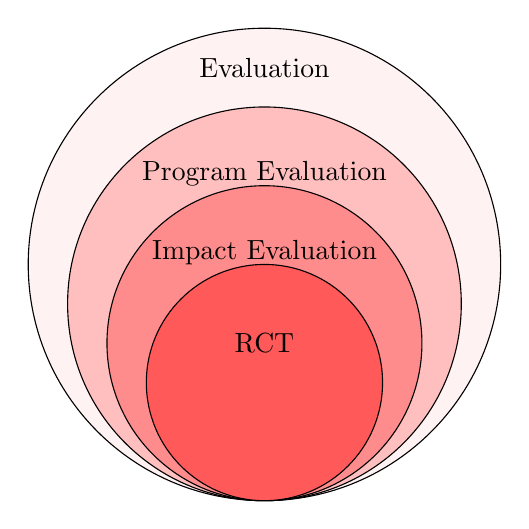
\begin{tikzpicture}
			\begin{scope}
				\coordinate (O) at (0,0);
				\coordinate (1)	at (0,-0.5); 
				\coordinate (2) at (0,-1); 
				\coordinate (3) at (0,-1.5); 
				
				\draw[fill=red!5] 		(O) circle (3);
				\draw[fill=red!25] 	(1) circle (2.5);
				\draw[fill=red!45] 	(2) circle (2);
				\draw[fill=red!65] 	(3) circle (1.5);
				%\draw[step=1cm,gray,very thin] (-3,-3) grid (3,3);
				
				\node[align=center] at (0,-1) {RCT}; 
				\node[align=center] at (0,.15) {Impact Evaluation}; 
				\node[align=center] at (0,1.15) {Program Evaluation}; 
				\node[align=center] at (0,2.5) {Evaluation}; 
			\end{scope}
		\end{tikzpicture}
	\end{center}
\end{frame}
%------------------------------------------------
\begin{frame}
	\frametitle{¿Qué es lo que necesitamos?}

	\begin{itemize}
		\item Una pregunta que contestar:
		\item Una hipótesis (causal):
		
		\begin{itemize}
			\item Causa
			\item Efecto
			\item ¿Quiénes y cómo?
		\end{itemize}
	\end{itemize} 

\end{frame}
%------------------------------------------------
\begin{frame}
	\frametitle{Componentes de la evaluación de impacto}

	 \begin{itemize}
		 \item Valoración inicial
		 \begin{itemize}
			 \item ¿Cómo se ha creado la situación?
		 \end{itemize}
		 \item Teoría de cambio
		 \item Proceso de evaluación
		 \item Evaluación de impacto
		 \item Análisis de costo-efectividad
	 \end{itemize}

\end{frame}
%------------------------------------------------
\begin{frame}
	\frametitle{Data}

	\textbf{Data es: }
	\begin{itemize}
		\item Hermosa
		\item Perspicaz
		\item Potente
		\item Engañosa
	\end{itemize}
\end{frame}
%------------------------------------------------
\begin{frame}
	\frametitle{Data es perspicaz}
	Ebenstein et al. (2017)
	\begin{figure}[H]
		\centering
		\includegraphics[width=0.3\textwidth]{rdd_china.jpg}
	\end{figure}

\end{frame}
%------------------------------------------------
\begin{frame}
	\frametitle{Correlación no es causalidad}

	\begin{itemize}
		\item Correlación espuria
		\item Una historia causal tampoco es \textit{causalidad}
		\item Aún usando datos muy sofisticados no significa que los resultados sean causales
	\end{itemize}
	

\end{frame}
%------------------------------------------------
\begin{frame}
	\frametitle{Correlación no es causalidad}

	\begin{figure}[H]
		\centering
		\includegraphics[width=1\textwidth]{espurio.pdf}
	\end{figure}

\end{frame}
%------------------------------------------------
\section{Diferencias en diferencias}
\subsection{Diferencias en diferencias}
%------------------------------------------------
\begin{frame}
	\frametitle{DID}

	\begin{figure}
		\centering 
		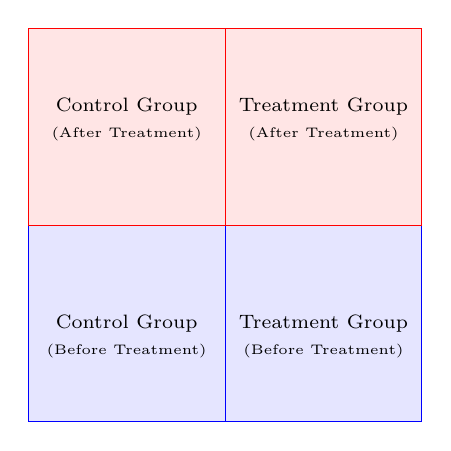
\begin{tikzpicture}
			\fill[blue!10!white, draw=blue]  (0,0) rectangle (2.5,2.5);
			\fill[blue!10!white, draw=blue]  (2.5,0) rectangle (5,2.5);
			\fill[red!10!white,  draw=red]  (0,2.5) rectangle (2.5,5);
			\fill[red!10!white,  draw=red]  (2.5,2.5) rectangle (5,5);
			
			\node at (1.25,1.25) {\scriptsize{Control Group}}; 
			\node at (1.25,4) {\scriptsize{Control Group}}; 
			\node at (3.75,4) {\scriptsize{Treatment Group}}; 
			\node at (3.75,1.25) {\scriptsize{Treatment Group}}; 
			
			\node at (1.25,.9) {\tiny{(Before Treatment)}}; 
			\node at (3.75,.9) {\tiny{(Before Treatment)}}; 
			
			\node at (1.25,3.65) {\tiny{(After Treatment)}}; 
			\node at (3.75,3.65) {\tiny{(After Treatment)}}; 
		\end{tikzpicture}
	\end{figure}

\end{frame}
%------------------------------------------------
\begin{frame}
	\frametitle{DID: Ejempplo de desempleo}

	\begin{figure}\centering
		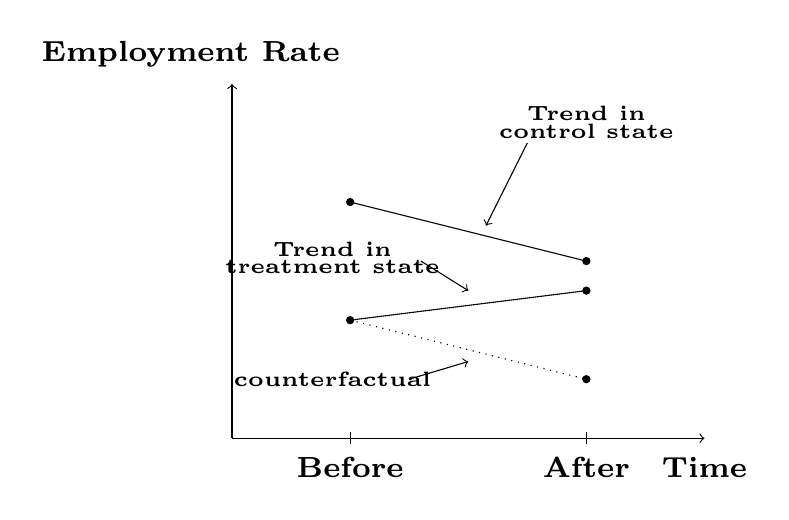
\begin{tikzpicture}[scale=1.5, transform shape]
			%\draw[step=0.5cm,gray,very thin] (0,0) grid (4,3);
			\draw[->] (0,0) -- (4,0) ; 
			\draw[->] (0,0) -- (0,3) ; 
			\draw[-] (1,2) -- (3,1.5); 
			\draw[dotted] (1,1) -- (3,0.5); 
			\draw[-] (1,1) -- (3,1.25);
			\draw[->] (2.5,2.5) -- (2.15,1.8);
			\draw[->] (1.6,1.5) -- (2,1.25); 
			\draw[->] (1.5,0.5) -- (2,0.65); 
			\draw[-] (1,0.05) -- (1,-0.05);
			\draw[-] (3,0.05) -- (3,-0.05);
			(3.1,1.25) -- node[right] {{\tiny Treatment Effect}} (3.1,0.5);
			\node at (4,-0.25) {\scriptsize\textbf{Time}};
			\node at (-0.35,3.25) {\scriptsize\textbf{Employment Rate}};
			\node at (1,-0.25) {\scriptsize\textbf{Before}};
			\node at (3,-0.25) {\scriptsize\textbf{After}};
			\node at (3,2.75) {\tiny\textbf{Trend in}};
			\node at (3,2.6) {\tiny\textbf{control state}};
			\node at (0.85,1.6) {\tiny\textbf{Trend in}};
			\node at (0.85,1.45) {\tiny\textbf{treatment state}};
			\node at (0.85,0.5) {\tiny\textbf{counterfactual}};
			\fill (1,1) circle[radius=1pt];
			\fill (3,0.5) circle[radius=1pt]; 
			\fill (3,1.5) circle[radius=1pt]; 
			\fill (3,1.25) circle[radius=1pt]; 
			\fill (1,2) circle[radius=1pt]; 
		\end{tikzpicture}
	\end{figure} 
\end{frame}
%------------------------------------------------
\begin{frame}
	\frametitle{Importancia del estudio: background y contexto}

	\begin{itemize}
		\item Incremento de una política (aumento del salario mínimo).
		\item New Jersey v. Pennsylvania -- NJ es una estado relativamente pequeño y con una economía ligada a otros estados.
		\item Patrones similares de empleo en NJ y PA Este.
		\item Card y Krueger (1992) siguieron approx. 100 por ciento de las ventas, de la primera ronda, en la segunda ronda.  
	\end{itemize}
\end{frame}
%------------------------------------------------
\begin{frame}
	\frametitle{Conclusión del paper}

	\begin{itemize}
		\item Salario mínimo $\uparrow$ ; Empleo $\uparrow$
		\item La carga del salario mínimo pasó a los consumidores.
		\item No hubo evidencia que precios aumentaros más en los locales que se vieron afectados por el incremento del salario mínimo.
	\end{itemize}

\end{frame}
%==============================================================
\miniframesoff 	
\begin{frame}[plain, noframenumbering]
	\begin{center}
	\LARGE STATA TIME
		\begin{figure}[H]
			\includegraphics[width=0.57\textwidth]{stata.pdf}
		\end{figure}
	\end{center}
\end{frame}
%==============================================================
% END
%==============================================================	
\begin{frame}[plain, standout]
	Nos vemos mañana.
\end{frame}
%-----------------------------------------------
\end{document}		
